\iffalse
\begin{figure}[h]
\centering
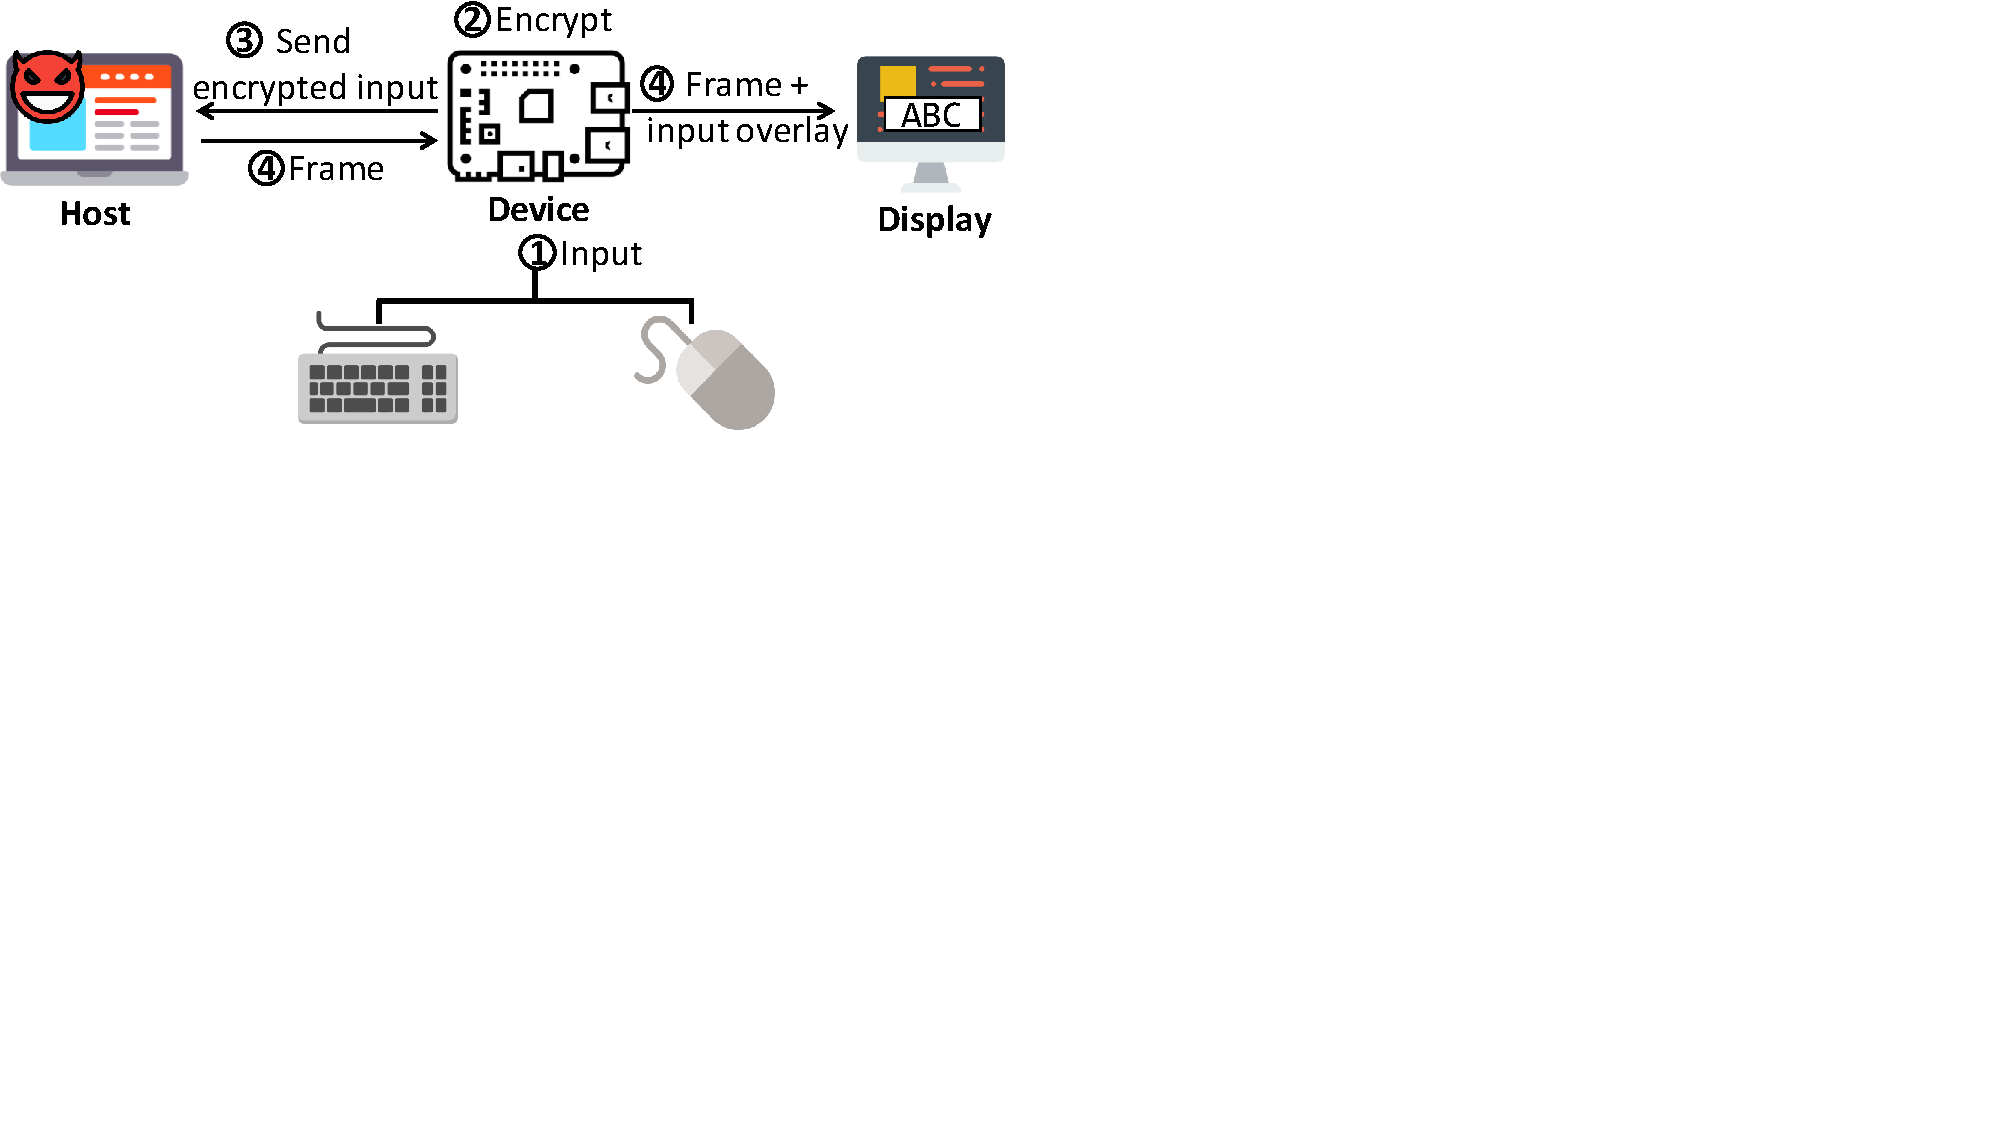
\includegraphics[trim={0 11cm 16.5cm 0}, clip, width=\linewidth]{inputPrivacy.pdf}
\caption{Input Confidentiality}
\label{fig:inputPrivacy}
\centering
\end{figure}
\fi



\section{Input \& Output Confidentiality}
\label{sec:confidentiality}


In the previous sections (the main protocol is described in Section~\ref{sec:systemDesign:mainProtocol}), we describe how the \name \js and the \device together transform and overlay the UI to ensure the integrity of the UI and the input data. Minor modification can be made to this method to introduce confidentiality to all IO. One of the major components for achieving IO confidentiality is to establish a secure channel between the server and the \device. Using this \tls channel, the remote server sends all the UI elements to the \device and the \device submits all user inputs to the remote server.

\subsection{Establishing \tls}
\label{sec:confidentiality:tls}

\begin{figure}[t]
\centering
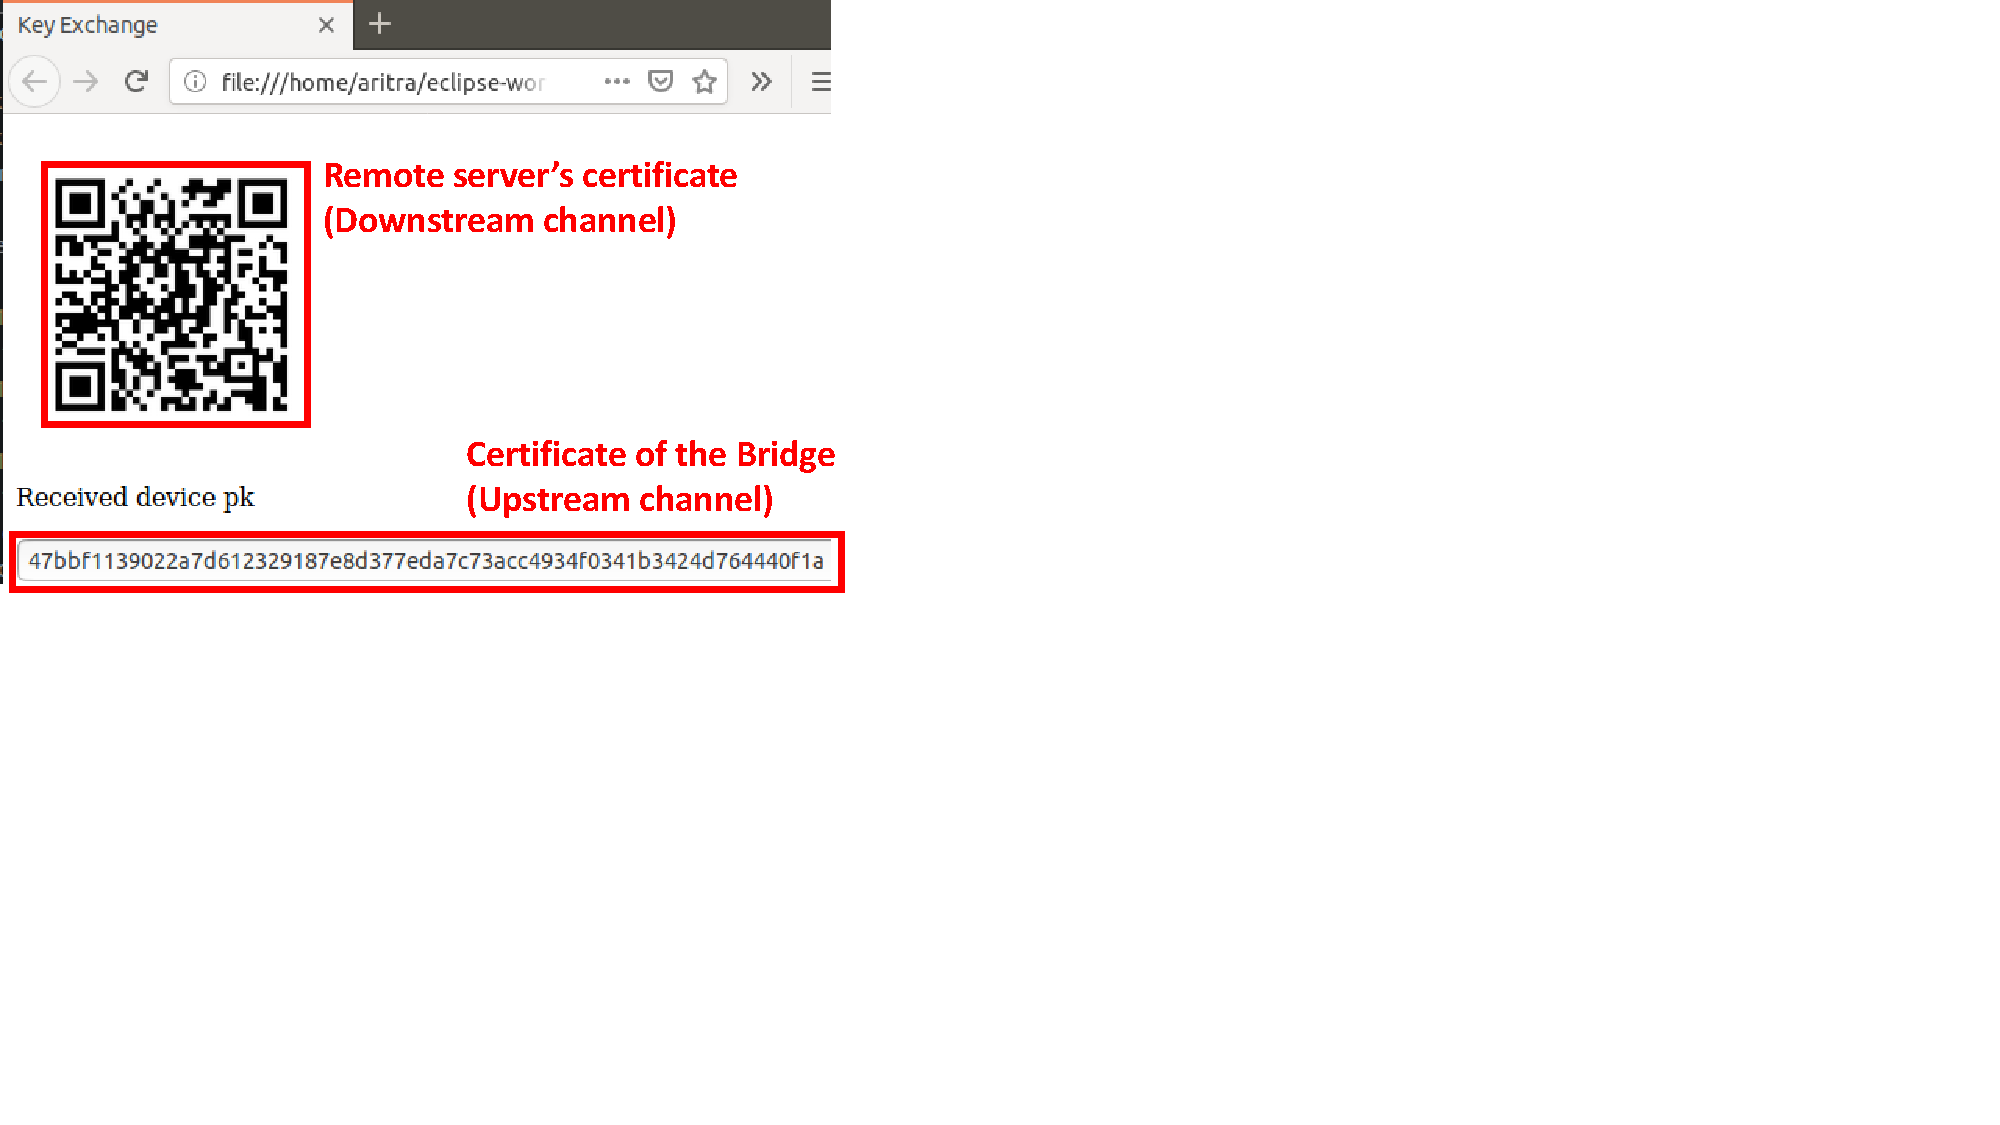
\includegraphics[trim={0 8cm 18cm 0}, clip, width=0.85\linewidth]{keyExchange.pdf}
\caption{\textbf{Key establishment.} A snapshot of the key exchange web page that is used to communicate the public certificates of the device and the remote server. This page only lasts for a few milliseconds. Hence the page is practically invisible to the user. The QR-code displayed on the web page serves as the downstream channel from the remote server to the \device, whereas the text field is the upstream channel.}
\spacesave
\label{fig:keyExchange}
\centering
\end{figure} 


When the user opens up a webpage that supports \name mechanism, key exchange is the first step that is executed by the \device. Also, the key exchange phase is crucial as the remote server also decide if the user has a \device. We assume that the remote server already has the \device's certificate, or some offline registration takes place. An instance of the key exchange mechanism of \name is illustrated in Figure~\ref{fig:keyExchange}. The flow of the key exchange mechanism is as the following:

\begin{mylist}
  \item The remote web server serves the web page that shows a QR code that encodes the signed public key of the remote server (server hello in TLS). This page has a $5$ seconds timeout.
  \item The device captures the frames and looks for a QR code. As soon as the device finds one, the device decodes the QR code and verifies it.
  \item If the verification is successful, the device emulates itself as a keyboard device to the host system. The device then encodes its signed public certificate to hexadecimal and send it as a keystroke to the host (client hello in the TLS). For signature, the \device uses the root key of the device manufacturer.
  \item The \name  JavaScript snippet looks for the keystrokes, and as soon as it gets a string of a specific length, it sends the key strokes to the remote server, and the \name JavaScripts loads the webpage.
  \item In case the user does not have a \device, the step mentioned above does not take place within the $5$ seconds timeout period. In that case, \name JavaScript snippet concludes that the user does not have a \device. This allows the webpage to fallback to conventional web UIs that do not involve \device for their operation.
\end{mylist}

After this, both the device and the remote server have each other's public certificates. Using these certificates, both the \device and remote server calculates the shared secret using the authenticated Diffie-Hellman protocol~\footnote{Assume that $(g^x, x)$ and $(g^y, y)$ is the public-private key pair of the remote server and the \device respectively, where $g$ being a generator of a group $G$. The remote server sends a QR code that encodes a CA-signed $g^x$. The \device transmits signed $g^y$ to the remote server. Both the remote server and the \device computes $g^{xy}=(g^x)^y=(g^y)^x$ as the shared secret. Detailed description can be found  in~\cite{blake1998authenticated}.}.




\lstset{language=HTML, frame=tb, caption=\small{\textbf{HTML page from the remote server that contains the encrypted UI specification for IO confidentiality.}} , label = snippet:encryptedHTML, firstnumber =1}
\begin{figure}[t]
\small
\begin{lstlisting}[mathescape=true]
<form action="/some_action">
  Text box 1:<br>
  <input type="text" name="text_box_1">
  <br> text box 2:<br>
  <input type="text" name="text_box_2">
  <encrypted_qr><!-encrypted UI specification->
  0x4a5c4... </encrypted_qr>
  <script> [JS outputs QR code that encodes 
  encrypted specification] </script>
</form> 
\end{lstlisting} 
\end{figure}



\begin{figure}[t]
\centering
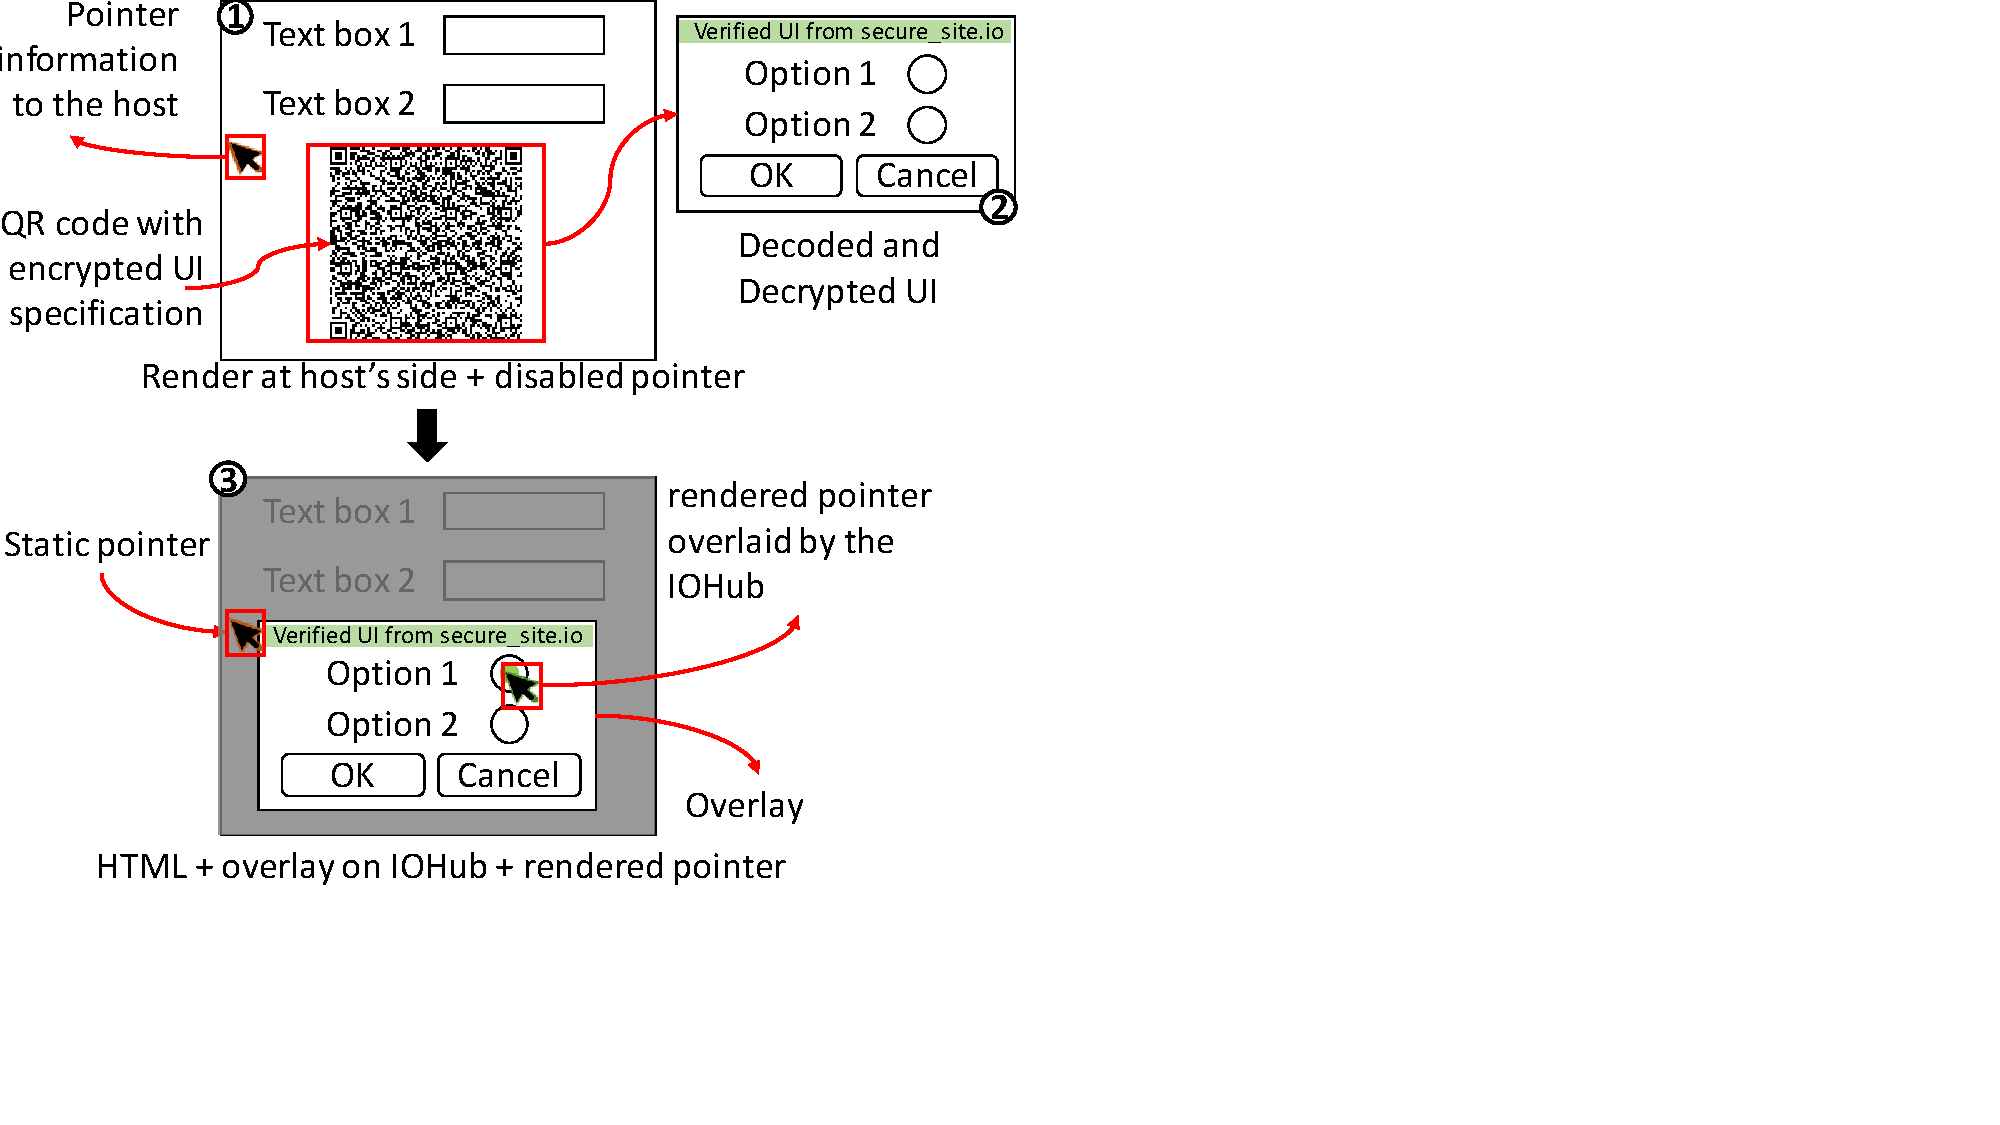
\includegraphics[trim={0 3cm 16.5cm 0}, clip, width=0.88\linewidth]{activityPrivacyRender.pdf}
\caption{\textbf{IO confidentiality.} The figure shows how \name achieves the confidentiality of the UI elements and the mouse pointer in the presence of a compromised host. The upper screenshot shows the host's view of the display while the lower one shows the user's view. The host can only see a QR code where the specification is encrypted by the \tls session key between the \device and the remote server. The user saw the decoded and overlaid UI objects that are retrieved from the QR code sent by the remote server (as described in Section~\ref{sec:systemDesign:transformation}).}
\spacesave
\label{fig:activityPrivacy}
\centering
\end{figure}

After the server and the \device establish the \tls channel, \name is ready to provide IO confidentiality.

\myparagraph{Output confidentiality} Output confidentiality ensures that no information sent from the remote server is visible to the host. To enable output confidentiality, the UI overlay mechanism that is described in Section~\ref{sec:systemDesign:transformation} is modified slightly. Here we \name does not require \name JS to transform all the UI elements to QR code specification. A small server-side module that is very similar to \name JS transforms the UI elements to the UI specification (one such specification is provided in Specification~\ref{snippet:UISpecification}) and encrypt the specification with the \tls session key (Section~\ref{sec:confidentiality:tls}). The \device decodes the QR code from the intercepted HDMI frames, decrypts the specification and overlays the UI on the HDMI frames. One example is provided in the HTML Snippet~\ref{snippet:encryptedHTML} where the \texttt{<encrypted>} tag contains the encrypted UI specification from the server. The \name JS (inside \texttt{<script>} tag) encodes this encrypted UI specification to a QR code.

\myparagraph{Input Confidentiality} When the user enters her mouse pointer into the overlaid UI boundary, the \device stops transmitting any mouse data to the output system, making the host completely oblivious to any mouse movement done by the user. Likewise, when the user selects a UI element, for example, a radio button that is shown in Figure~\ref{fig:activityPrivacy}, the \device encrypts and signs the packets and sends the packet to the remote server making the input commands/values hidden from the attacker-controlled host.  

